\apendice{Especificación de diseño}

\section{Introducción}
Este apéndice describe el diseño detallado de la aplicación FutboStats. FutboStats es una aplicación web que permite a los usuarios buscar información sobre partidos de fútbol, equipos, y competiciones, así como consultar estadísticas avanzadas y predicciones. Este documento cubre el diseño de datos, el diseño procedimental y el diseño arquitectónico de la aplicación.

\section{Diseño de datos}
FutboStats no utiliza una base de datos persistente, sino que se basa en la interacción con API-FOOTBALL y la API en Flask para obtener los datos necesarios. Los datos se manejan de la siguiente manera:
\subsection{Estructura de solicitudes y respuestas de API-FOOTBALL}
Las solicitudes a la API-FOOTBALL se estructuran en formato JSON y contienen parámetros como el nombre del equipo, nombre de la liga o fecha del partido. Estas solicitudes requieren incluir una clave de API (\textit{API key}) y un host de API (\textit{API host}) en los encabezados para autenticación. Cada endpoint de la API tiene parámetros establecidos, algunos de los cuales son opcionales.
Para acceder a API-FOOTBALL, es necesario incluir en cada solicitud los siguientes encabezados:
\begin{itemize}
    \item \textbf{API key:} Clave única proporcionada al registrarse en la API-FOOTBALL, utilizada para autenticar las solicitudes.
    \item \textbf{API host:} Identificador del host de la API, que especifica el servidor al cual se envían las solicitudes.
\end{itemize}
Cada endpoint de la API-FOOTBALL acepta diferentes parámetros, que pueden ser obligatorios u opcionales. Algunos de los parámetros comunes incluyen:
\begin{itemize}
    \item \textbf{Identificador del equipo:} identificador del equipo para el cual se desean obtener datos.
    \item \textbf{Identificador de la liga:} identificador de la liga para la cual se quieren obtener estadísticas o clasificaciones.
    \item \textbf{Fecha:} fecha del partido para el cual se desean obtener los resultados o detalles.
    \item \textbf{Season:} año de la temporada por la que se desea filtrar la información.
\end{itemize}
A continuación, en la figura C.1 se muestra un ejemplo de cómo se estructura una solicitud en formato JSON realizada mediante la herramienta Postman:

\begin{figure}[H]
    \centering
    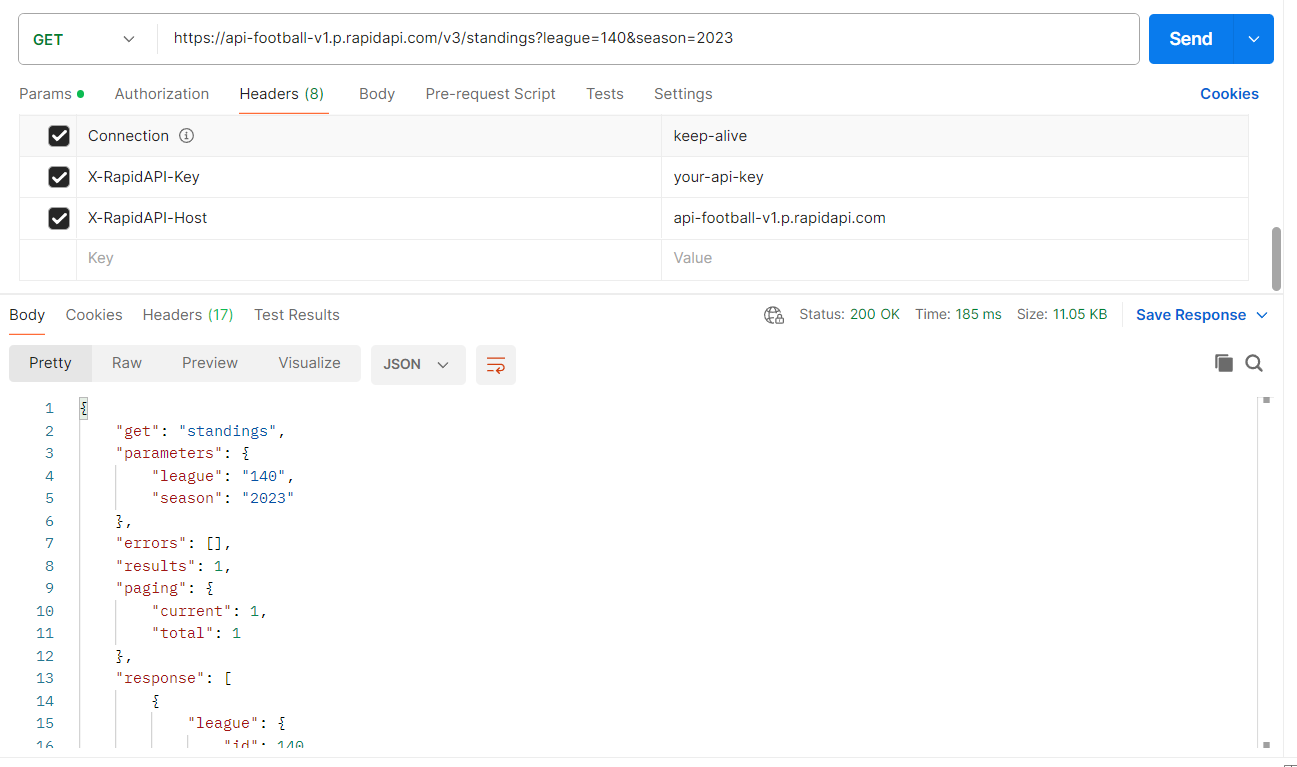
\includegraphics[width=1\linewidth]{img/ejemploPostman.png}
    \caption{Ejemplo de petición a API-FOOTBALL}
    \label{fig:enter-label}
\end{figure}

Como podemos ver se realiza una petición GET al \textit{endpoint} '/standings' para obtener una clasificación en concreto. Le pasamos como parámetros el identificador de liga 140(es el identificador de La Liga española) y la season 2023(año de la clasificación). Para que la petición tenga éxito tenemos que establecer en los headers el campo 'X-RapidAPI-Key' con la Api-key que da API-FOOTBALL al registrarse y el campo 'X-RapidAPI-Host' con el host correspondiente que en mi caso es 'api-football-v1.p.rapidapi.com'. Como podemos observas en el body observamos el resultado en JSON de la petición GET y el status de la petición que ha sido un 200 OK.
\subsection{Estructura de solicitudes y respuestas de la API en Flask}
La API diseñada en Flask contiene varios \textit{endpoints}. Algunos devuelven un JSON con la información del modelo de goles esperados o con la información de la tablas de los puntos esperados. En cambio, otros devuelven imágenes generadas en Python utilizando los datos de StatsBomb.\\
En la figura C.2 muestro un ejemplo de petición a la API creada en Flask:

\begin{figure}[H]
    \centering
    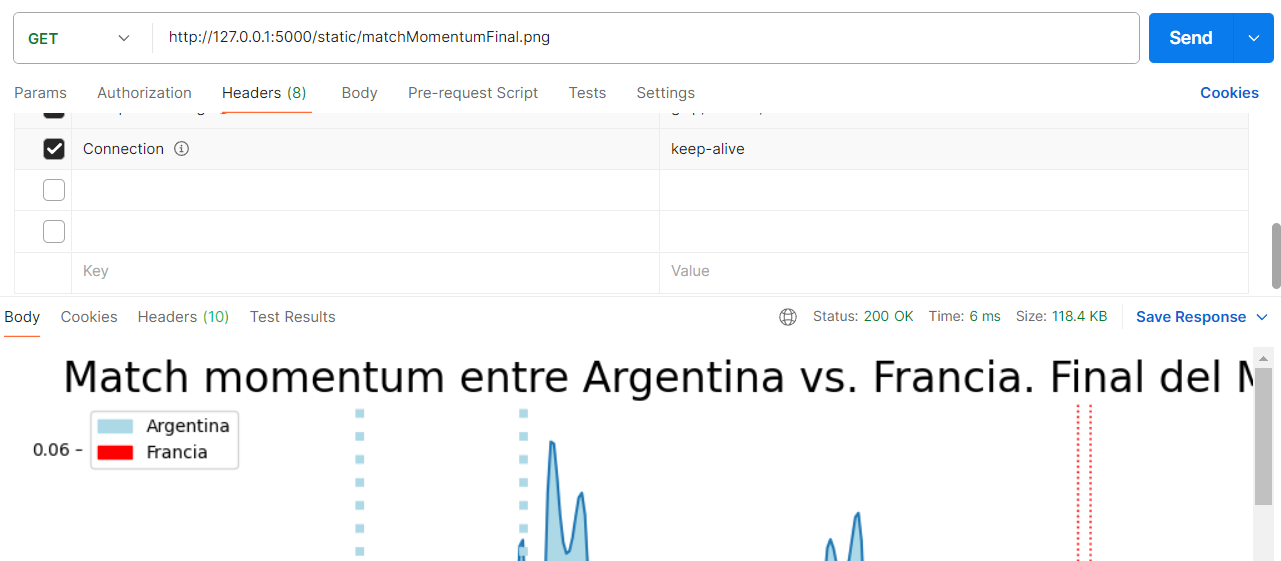
\includegraphics[width=1\linewidth]{img/ejemploPostman2.png}
    \caption{Ejemplo de petición a la API de Flask}
    \label{fig:enter-label}
\end{figure}

Como podemos ver en la imagen, se realiza una petición a un \textit{endpoint} que devuelve una imagen. En este caso basta con hacer la petición al \textit{endpoint} correcto sin utilizar una Api-key.

\subsection{Manejo de datos en memoria}
Los datos recibidos de la API se almacenan temporalmente en la memoria del cliente \textit{(front-end)} para su visualización y en el servidor (\textit{back-end}) para el procesamiento de predicciones y seguimiento de jugadores con ImageAI. \\
Cuando se realiza una petición a la API-FOOTBALL desde el \textit{front-end} desarrollado en Angular, los datos recibidos se almacenan en memoria en el cliente. Esto permite que la aplicación web pueda mostrar rápidamente la información solicitada por el usuario sin necesidad de realizar repetidas consultas a la API. Los datos en memoria se gestionan mediante servicios de Angular que mantienen el estado de la aplicación. \\
Cuando se realiza una petición al \textit{back-end}, los datos también se manejan en memoria temporalmente. Además, los datos procesados, como gráficos e imágenes, se guardan en las carpetas 'static' y 'uploads'. La carpeta static almacena imágenes de los gráficos generados, mientras que la carpeta uploads se utiliza para almacenar los vídeos procesados. \\
En resumen, los datos de la API-FOOTBALL se almacenan temporalmente en la memoria del frontend Angular para una rápida visualización y se manejan en memoria en el \textit{back-end} Flask para el procesamiento de predicciones y vídeos, guardando los resultados en las carpetas 'static' y 'uploads'.

\section{Diseño procedimental}
En esta sección se describen los flujos de trabajo y procedimientos clave en FutboStats.

\subsection{Flujo de búsqueda de datos en API-FOOTBALL}
\begin{enumerate}
	\item El usuario ingresa los criterios de búsqueda (fecha, nombre del equipo, nombre de la liga).
	\item El \textit{front-end} envía una solicitud a API-FOOTBALL a través de los servicios de Angular.
        \item La API-FOOTBALL devuelve los datos a Angular.
        \item Angular procesa los datos y los envía a la vista.
        \item Se muestran los resultados al usuario.
\end{enumerate}

\begin{figure}[H]
    \centering
    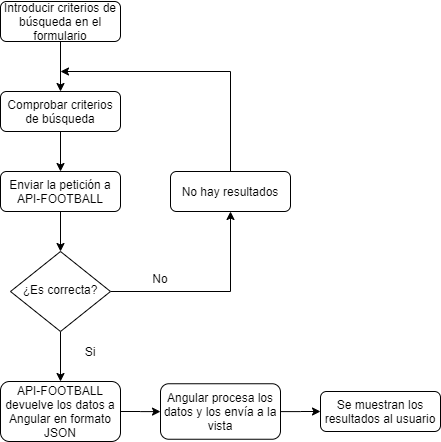
\includegraphics[width=0.7\linewidth]{img/flujo1.png}
    \caption{Diagrama de flujo de obtención de datos a API-FOOTBALL}
    \label{fig:enter-label}
\end{figure}


\subsection{Proceso de autenticación}
\begin{enumerate}
	\item El usuario selecciona la opción de iniciar sesión.
	\item El \textit{front-end} redirige al usuario al proveedor de autenticación (Google).
        \item El usuario se autentica y se redirige de vuelta al \textit{front-end} con un token.
        \item El \textit{front-end} valida el token utilizando las bibliotecas de autenticación de Google.
        \item Se crea una sesión para el usuario.
        \item El usuario puede acceder a las funcionalidades protegidas de la aplicación.
\end{enumerate}

\begin{figure}[H]
    \centering
    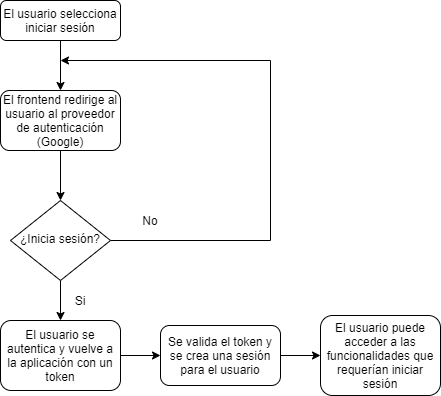
\includegraphics[width=0.7\linewidth]{img/flujo2.png}
    \caption{Diagrama de flujo de inicio de sesión en FutboStats}
    \label{fig:enter-label}
\end{figure} 

\subsection{Flujo de predicciones}
\begin{enumerate}
	\item El usuario inicia sesión y accede a la sección de predicciones.
	\item El \textit{front-end} envía una solicitud al \textit{back-end} para obtener los datos de las predicciones(goles esperados, puntos esperados, gráficos del mundial).
        \item El \textit{back-end} realiza cálculos utilizando los datos de la librería StatsBombPy.
        \item El \textit{back-end} devuelve los resultados del modelo al \textit{front-end}.
        \item El \textit{front-end} muestra las predicciones al usuario en forma de gráficos y tablas.
\end{enumerate}
\begin{figure}[H]
    \centering
    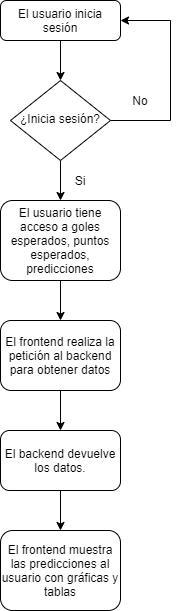
\includegraphics[width=0.3\linewidth]{img/flujo3.png}
    \caption{Diagrama de flujo de obtención de datos en la API de Flask}
    \label{fig:enter-label}
\end{figure}

\subsection{Procesamiento de vídeos para tracking}
\begin{enumerate}
    \item El usuario inicia sesión y accede a la sección de SportsAI.
    \item El usuario sube un vídeo a la aplicación.
    \item El \textit{front-end} envía el vídeo al \textit{back-end}.
    \item El \textit{back-end} procesa el vídeo utilizando el modelo de \textit{tracking} de ImageAI.
    \item El \textit{back-end} genera un vídeo procesado con el \textit{tracking} aplicado.
    \item El \textit{back-end} envía el vídeo procesado al \textit{front-end}.
    \item El \textit{front-end} muestra el vídeo procesado al usuario. 
\end{enumerate}

\begin{figure}[H]
    \centering
    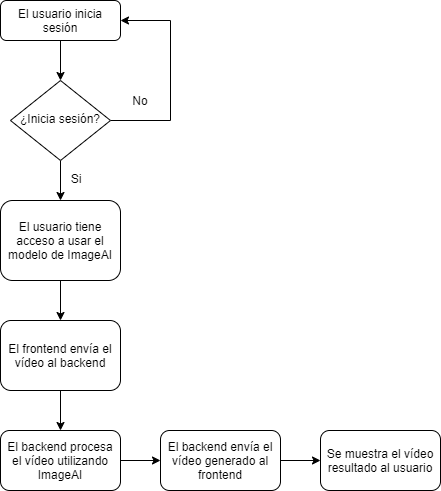
\includegraphics[width=0.7\linewidth]{img/flujo4.png}
    \caption{Diagrama de flujo de uso de ImageAI}
    \label{fig:enter-label}
\end{figure}

\section{Diseño arquitectónico}
FutboStats utiliza una arquitectura cliente-servidor porque divide claramente las responsabilidades entre el \textit{front-end} y el \textit{back-end}, se comunican a través de peticiones HTTP, y facilita la interacción con servicios externos, el procesamiento de datos y la independencia de plataforma \cite{web:clienteServidor}. El \textit{front-end} está desarrollado en Angular y el \textit{back-end} en Flask. La aplicación interactúa con la API-FOOTBALL para obtener los datos necesarios.
\subsection{Descripción general de la arquitectura}
La arquitectura de FutboStats se divide en dos capas principales: el \textit{front-end} y el \textit{back-end}. 
Tiene las siguientes características de una arquitectura cliente-servidor:
\begin{itemize}
    \item \textbf{Separación de responsabilidades:} en FutboStats, el \textit{front-end} (cliente) está desarrollado en Angular y se encarga de la interfaz de usuario y los servicios que hacen las peticiones a API-FOOTBALL, gestionando las interacciones del usuario y la presentación de los datos. El \textit{back-end} (servidor), desarrollado en Flask, maneja la lógica de negocio y el procesamiento de los datos, gráficos, imágenes y vídeos.
    \item \textbf{Comunicación a través de HTTP:} la arquitectura cliente-servidor implica que el cliente y el servidor se comuniquen a través de peticiones HTTP. En FutboStats, el frontend realiza peticiones HTTP al backend para obtener datos de predicciones, modelos, gráficos y este responde con la información pedida.
    \item \textbf{Independencia de plataforma:} esta arquitectura permite que el cliente y el servidor se ejecuten en plataformas diferentes. El \textit{front-end} puede ser accedido desde cualquier navegador web (desplegado en Netlify), mientras que el \textit{back-end} puede estar alojado en un servidor remoto(desplegado en Render). Esta separación facilita la escalabilidad y el mantenimiento de la aplicación.
    \item \textbf{Procesamiento de datos en el servidor:} el procesamiento de predicciones, generación de gráficos y el tracking de vídeos, se realizan en el \textit{back-end}. Esto descarga al cliente de tareas intensivas en recursos y permite una mayor eficiencia y seguridad en el manejo de datos.
\end{itemize}
En la figura C.7 se muestra la arquitectura cliente-servidor.
\begin{figure}[H]
    \centering
    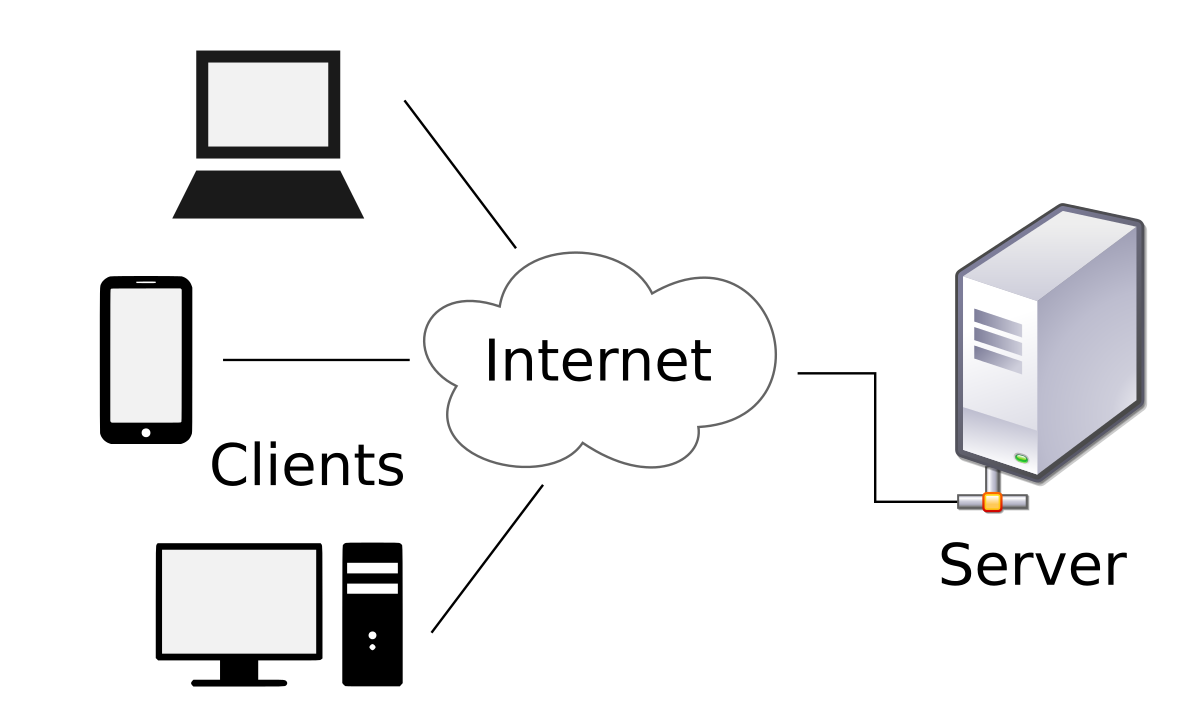
\includegraphics[width=0.7\linewidth]{img/cliente-servidor.png}
    \caption{Arquitectura cliente-servidor \cite{web:clienteServidor2}}
    \label{fig:enter-label}
\end{figure}

\subsection{Componentes principales}
\textbf{Frontend (Angular):}
\begin{itemize}
    \item Componente de búsqueda: permite a los usuarios buscar partidos, equipos y clasificaciones mediante la interacción del usuario.
    \item Componente de visualización: muestra los resultados de búsqueda y estadísticas mediante tablas y tarjetas.
    \item Componente de autenticación: gestiona el inicio de sesión de los usuarios.
    \item Servicios que manejan las peticiones a API-FOOTBALL.
\end{itemize}
\textbf{Backend (Flask):}
\begin{itemize}
    \item Módulo de predicciones: calcula las predicciones de puntos esperados y goles esperados.
    \item Generación de gráficos: se generan gráficos con los datos de StatsBombPy que son guardados en la carpeta 'static'.
    \item Módulo de procesamiento de videos: procesa los vídeos utilizando ImageAI.
\end{itemize}

\section{Diseño de interfaces}
En el diseño de la interfaz se han realizado varios prototipos inicialmente utilizando la aplicación \textit{JustInMind}. Estos primeros prototipos sirvieron para definir la paleta de colores que iba a usar la aplicación (verde, blanco y negro) y la distribución de las opciones del menú. \\
Las siguientes figuras muestran algunos prototipos que fueron desarrollados con \textit{JustInMind}:

\begin{figure}[H]
    \centering
    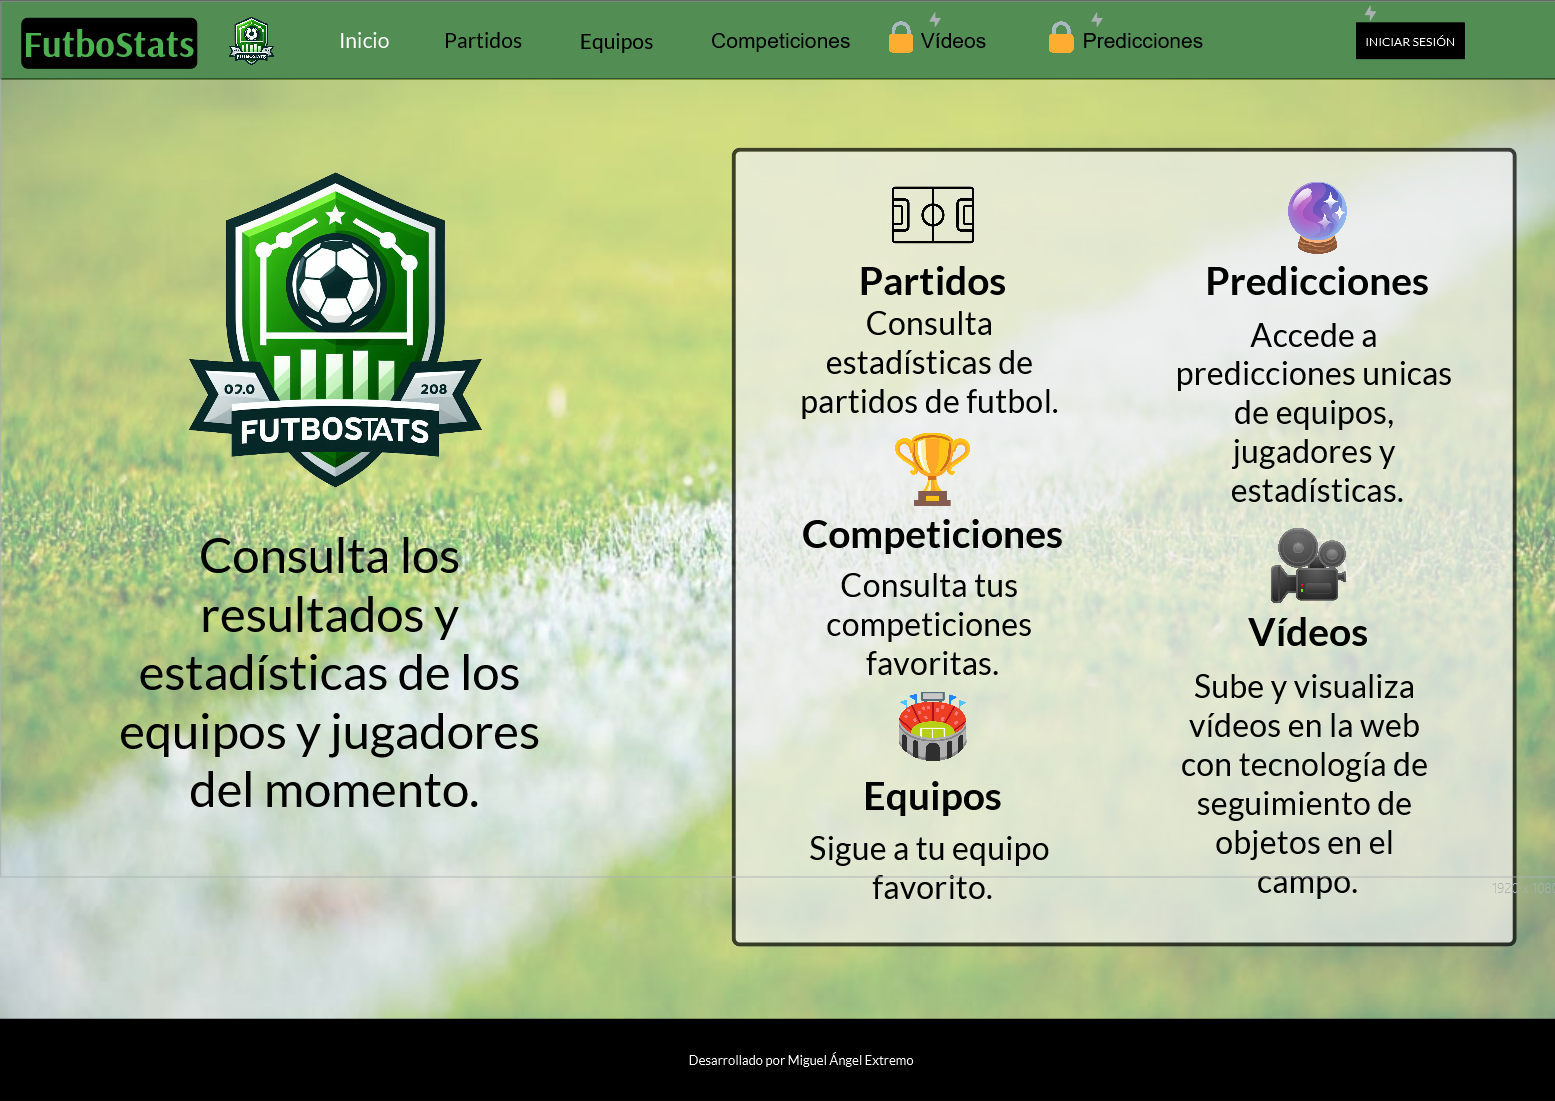
\includegraphics[width=0.7\linewidth]{img/prototipo.png}
    \caption{Prototipo de Inicio}
    \label{fig:enter-label}
\end{figure}

\begin{figure}[H]
    \centering
    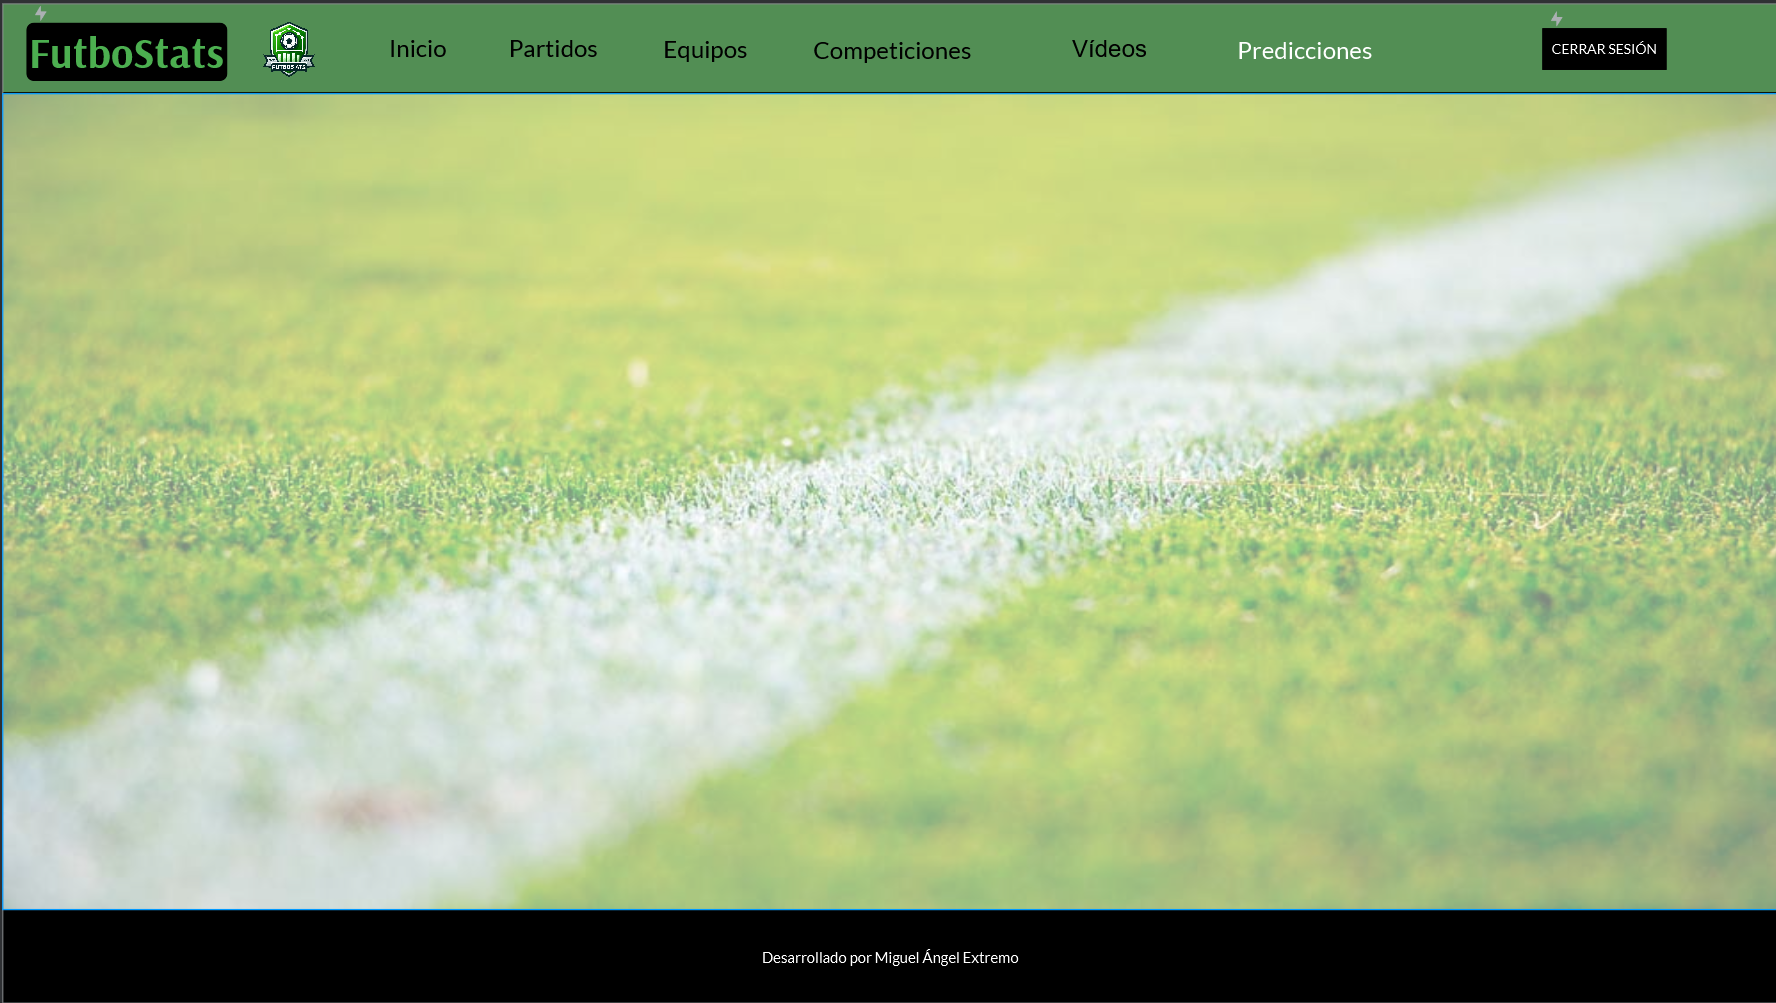
\includegraphics[width=0.7\linewidth]{img/prototipo3.png}
    \caption{Prototipo general con header, body y footer}
    \label{fig:enter-label}
\end{figure}

\begin{figure}[H]
    \centering
    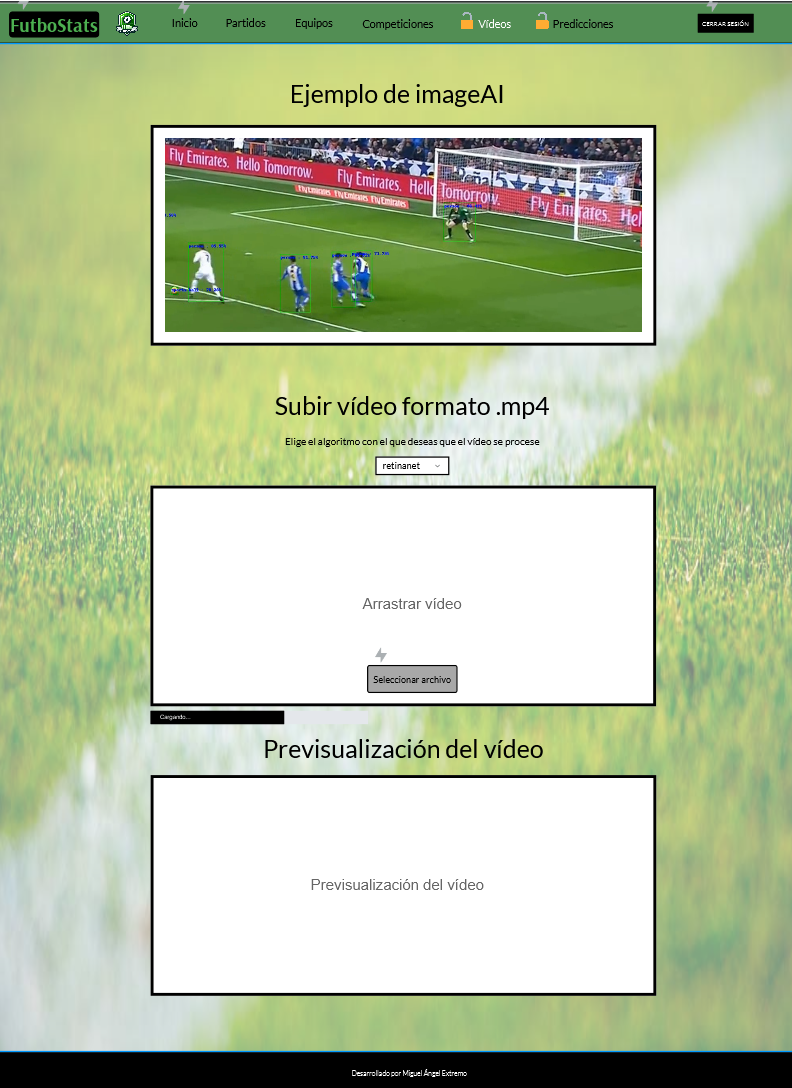
\includegraphics[width=0.7\linewidth]{img/prototipo2.png}
    \caption{Prototipo de la vista de ImageAI}
    \label{fig:enter-label}
\end{figure}

